\documentclass{llncs}
\usepackage{tikz}
\usepackage{amsfonts}
\usepackage{graphicx,url}
\usepackage[T1]{fontenc}
%\usepackage{psfig}
\usepackage{graphics}
\usepackage{amssymb,amsmath,latexsym}
\usepackage{listings} 
\usepackage{subfig}

%\newtheorem{theorem}{Theorem}[section]
%\newtheorem{theorem}{Theorem}[section]
%\newtheorem{example}[theorem]{Example}
%\newtheorem{algorithm}[theorem]{Algorithm}
%\newtheorem{definition}[theorem]{Definition}


\usepackage[thmmarks]{ntheorem}


\usepackage{listings}
\theoremstyle{plain}
\theoremheaderfont{\normalfont\bfseries}
\theorembodyfont{\normalfont}
\theoremseparator{.}
\theoremindent0cm
\theoremnumbering{arabic}
\theoremsymbol{\ensuremath{\Box}} 
\newtheorem{defi}{Definition}%[section]

\theoremheaderfont{\itshape}
\newtheorem{examp}{Example}%[section]

\theoremstyle{plain}
\theoremheaderfont{\normalfont\bfseries}
\theorembodyfont{\normalfont}
\theoremseparator{}
\theoremindent0cm
\theoremnumbering{arabic}
%\theoremsymbol{\ensuremath{\Box}} 
\newtheorem{algo}{Algorithm}%[section]

\theoremstyle{plain} 
\theoremsymbol{\ensuremath{\Box}} 
\theoremseparator{.} 
\newtheorem{prop}{Property}


\lstset{numbers=right, numbersep=5pt, numberstyle=\tiny, stepnumber=1,escapechar=\!,columns=fullflexible,
        morekeywords={procedure,let,for,do,if,then,else,add,choose,end,while,
        true,false,rise,exception,extend,resume,to,return,function}}



\def\B{\hfill{$\Box$}}
\def\A{\hbox{${\cal A}$}}
\def\P{\hbox{${\cal P}$}}
\def\T{\hbox{${\cal T}$}}
\def\O{\hbox{${\cal O}$}}
\def\W{\hbox{${\cal W}$}}
\def\useOpt{\hbox{${has\_opt}$}}


\def\bigS{\hbox{${\cal S}$}}
\def\bigSd{\hbox{${\cal S}_D$}}
\def\bigSsm{\hbox{${\cal S}_D^{score}$}}

\newcommand{\ie}{\ifmmode \mathit{i.e.}\else \textit{i.e.}\fi}
\newcommand{\wrt}{\ifmmode \mathit{w.r.t.}\else \textit{w.r.t.}\fi}
\newcommand{\eg}{\ifmmode \mathit{e.g.}\else \textit{e.g.}\fi}
\newcommand{\tuple}[1]{\ifmmode \langle #1 \rangle\else $\langle #1 \rangle$\fi}

\usepackage{authblk}

\begin{document}
%
% --- Author Metadata here ---

% --- End of Author Metadata ---
 
\title{Supporting Non-Functional Requirements for Services Software Process: An MDD Approach}

\author{Valeria de Castro\inst{1} \and Martin A. Musicante\inst{2} \and Umberto Souza da Costa\inst{2} \and Pl�cido~A.~de~Souza~Neto\inst{3} \and Genoveva Vargas-Solar\inst{4}}

\institute{Universidad Rey Juan Carlos -- M\'{o}stoles, Spain\\  \email{Valeria.deCastro@urjc.es} 
\and Federal University of Rio Grande do Norte (UFRN) -- Natal-RN, Brazil\\
\email{\{mam,umberto\}@dimap.ufrn.br}
\and Federal Institute of Rio Grande do Norte (IFRN) -- Natal-RN, Brazil\\ \email{placido.neto@ifrn.edu.br}
\and French Council of Scientific Research (CNRS) -- Grenoble, France\\
\email{Genoveva.Vargas-Solar@imag.fr}
}


 
\maketitle
\begin{abstract}
This paper presents an extension to the Service Oriented Development Method (SOD-M) to support the representation of some non-functional requirements. 
Specifically, we propose to extend SOD-M with: 
\textit{(i)} meta-models for representing non-functional requirements in different abstraction levels; 
\textit{(ii)} model to model transformation rules, useful to semi-automatically refine Platform Independent Models into Platform Specific Models; and 
\textit{(iii)} rules to transform Platform Specific Models into concrete implementations. 
We apply our proposal to develop a proof-of-concept example.
\end{abstract}

% A category with the (minimum) three required fields
%\category{H.4}{Information Systems Applications}{Miscellaneous}
%A category including the fourth, optional field follows...
%\category{D.2.8}{Software Engineering}{Metrics}[complexity measures,
%performance measures]

%\terms{Delphi theory} 

\keywords{MDD, Service Oriented Applications, Non-functional Properties}

\section{Introduction}

Model Driven Development (MDD) is top-down approach for the design and development of software systems. 
The main ideas of MDD were originaly proposed by the Object Management Group
(OMG)~\cite{mda}. 
MDD provides a set of
guidelines for the structuring of specifications.
The technique advocates for the use of \textit{models} to specify a software system at different levels of abstraction.
Abstraction levels are called \textit{viewpoints}. 
MDD defines three viewpoints:

\begin{trivlist}
\item \textbf{Computation Independent Models (CIM):} This level focusses on the
environment of the system, as well as on its business and requirement specifications. 
This viewpoint represents the software system at its highest level of abstraction. 
At this moment of the development, the structure and system processing details are still unknown or undetermined. 
 
\item \textbf{Platform Independent Models (PIM):} This level focusses on the system functionality, hiding the details of any particular platform. 
The specification defines those parts of the system that do not change from one platform to another. 

\item \textbf{Platform Specific Models (PSM):} This level focusses on the functionality, in the context of a particular implementation platform.
Models at this level combine the platform-independent view with the specific aspects of the platform to implement the system.  
\end{trivlist}

Besides the notion of model at each level of abstraction, MDD requires the use of \textit{model transformations} between levels.
These transformations may be automatic or semi-automatic and implement the refinement process between levels.

\bigskip 

In Service-Oriented Computing~\cite{Papazoglou2007}, pre-existing services are
combined to produce applications and provides the business logic. The selection of services is usually guided by the functional requirements of the application being developed. 
Some methodologies and techniques have been proposed to help the software
developer in the specification of functional requirements of the business logic,
such as the Service Oriented Development Method
(SOD-M)~\cite{decastro1}. 
SOD-M is based on MDD and proposes
models, practices and techniques to aid in software development. SOD-M does not
provide suport to the specification of non-functional requirements, such as
security, reliability, and efficiency. Ideally, non-functional requirements
would be considered along with all the stages of the software development. The
adoption of non-functional specifications from the early states of development
can help the developer to produce applications that are capable of dealing with
the application context.

\bigskip

Non-functional properties of service oriented applications have been
addressed in academic works and standards~\cite{ws-co,ws-tra,wsci}.
Dealing with these kind of properties involves the use of specific technologies
in different layers of the SOC architecture, for instance during the description
of services APIs (such as WSDL\cite{wsdl} or REST~\cite{rest}) or to express
service coordinations (like WS-BPEL~\cite{bpel03}).

%Existing work addressing non-functional properties for service-oriented applications can be classified under four approaches:
%\begin{trivlist}
%\item[-] Those coming from the Business Process Domain and from the Web
%service standards that propose ad-hoc protocols. 
%Examples of these include the WS*-Family of the W3C\cite{ws-co,ws-tra,btp}.
%\item[-] Those adopting a classic middleware approach were non-functional
%properties are provided as middleware services, like the ones presented
%in~\cite{BeVaC00,RohmBSS02,NepalFGJKS05,Bonita}.
%\item[-] Those providing languages and enabling the specification of protocols
%used for expressing service
%compositions~\cite{LakhalKY05,LakhalKY05b,RouachedGABG06,FauvetDDB05}.
%\item[-] Those adopting separation of concerns,
%like~\cite{Milanovic06,Espinosa-OviedoVZC09,SchmelingCM11,PastranaPK11}.
%\end{trivlist}

Protocols and models implementing non-functional properties assume the existence of a global control of the artifacts implementing the application.
They also assume that each service exports its interface.
So, the challenge of supporting non-functional properties is related to
\textit{(i)} The specification of the business rules of the application; and 
\textit{(ii)} Dealing with the technical characteristics of the infrastructure where the application is executed.

%In this context, there is a need of 
%\textit{(i)} flexible protocols and models accepting a best effort approach for ensuring non-functional properties.
%\textit{(ii)} A methodology for specifying the application logic and its associated non-functional properties, starting at the early phases of the development process.
%
%In this work, we proppose to address the structured engineering of service-oriented applications in the presence of non-functional properties where: 
%\textit{(i)} The designer must make the diference between requirements that concern the application logic and the non-functional requirements;
%\textit{(ii)} General concepts must be provided to support the representation of  different non-functional requirements;
%\textit{(iii)} The non-functional requirements, specified in an abstract way, must provide enough information to be translated into the specification of technical aspects implementing concrete non-functional properties to be verified at runtime.


The main goals of our work are:
\textit{(i)} To propose a methodology for supporting the construction of service-oriented applications, taking into account both functional and non-functional requirements;
\textit{(ii)} To improve the construction process by providing an abstract view of the application and ensure the conformance to its specification;
\textit{(iii)} To reduce the programming effort through the semi-automatic generation of  models for the application, to produce concrete implementations from high abstraction models;


\bigskip
This paper is organized as follows:
Sections~\ref{sec:sodm} and~\ref{sec:pisodm} presents, respectively, the SOD-M method of service software process and our proposed extension to deal with non-functional requirements.
A proof of concept example is developed in Section~\ref{sec:poc}.
We conclude the paper by presenting some related work and final remarks.

\section{SOD-M}\label{sec:sodm}
The Service-Oriented Development Method (SOD-M)~\cite{decastro1}
proposes the usage of the MDD approach in the context of service-based applications.
SOD-M provides a framework with models and standards to express functionalities
of applications at a high-level of abstraction. SOD-M meta-models are organized 
into three levels: CIM (\textit{Computational Independent Models}), 
PIM (\textit{Platform Independent Models}) and PSM (\textit{Platform Specific Models}).

Two models are defined at the CIM level: \textit{value model} 
and \textit{BPMN model}. 
The PIM level models the entire structure of the application flow,
while, the PSM level provides transformations towards more specific platforms.
The PIM-level models are: \textit{use case}, \textit{extended use case}, \textit{service process} and
\textit{service composition}. The PSM level models are: \textit{web service interface}, \textit{extended composition service} and \textit{business logic}. 
These three levels have no support for describing non-functional requirements. 

The SOD-M approach includes transformations between models:
\textit{CIM-to-PIM, PIM-to-PIM} and \textit{PIM-to-PSM} transformations. Given
an abstract model at the CIM level, it is possible to apply transformations for
generating a model of the PSM level. In this context, it is necessary to
follow the process activities described by the methodology. 

SOD-M considers two points of view:
\textit{(i)} \textit{business}, focusing on the characteristics and requirements
of the organization, and \textit{(ii)} \textit{system requirements}, focusing on
features and processes to be implemented in order application requirements. In
this way, SOD-M aims to simplify the design of service-oriented applications, as
well as its implementation using current technologies.


\section{$\pi$SOD-M}\label{sec:pisodm}

%In this section we present $\pi$SOD-M, an MDD based methodology. 
$\pi$SOD-M provides an environment for building service compositions considering
their non-functional requirements. 
$\pi$SOD-M extends the SOD-M meta-models by adding
the concept of \textit{Policy}~\cite{Espinosa-Oviedo2011a}
to represent non-functional requirements.

\begin{figure}[h]
\centering
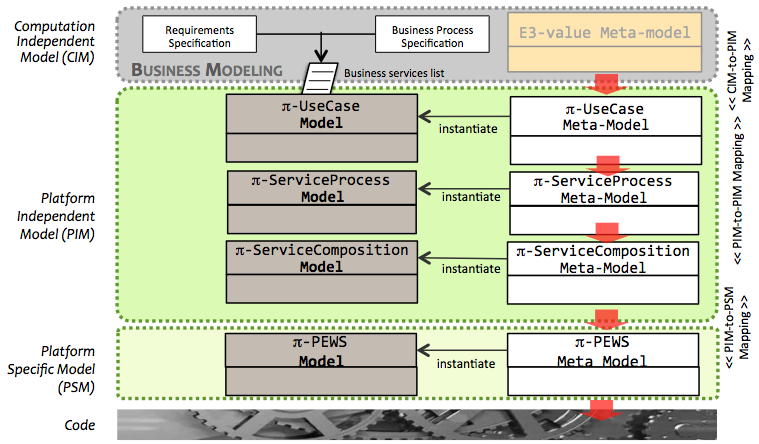
\includegraphics[width=1.0\textwidth]{figs/piSODM}
\caption{$\pi$SOD-M.}
\label{fig:piSOD-M}
\end{figure}

$\pi$SOD-M proposes the generation of a set of models at different abstraction levels, as
well as transformations between these models.
$\pi$SOD-M models represent both the functional aspects of the application as well as its non-functional constraints. 
Constraints are restrictions that must be verified during the execution of the application. 
An example of this is the requirement of the user's authentication for executing some system functions. 

Similarly to SOD-M, our approach targets the construction of service-oriented applications that implement business processes.
$\pi$SOD-M proposes a development process based on the definition of models
(instances of the meta-modes) and transformations between models.
There are two kinds of transformations:
Model-to-model transformations are used during the software process to refine the specification.
Model-to-text transformations are the last step of the process and generate code.

We extended SOD-M to include non-functional specifications.
Our method defines four meta-models: \textit{$\pi$-UseCase}, \textit{$\pi$-ServiceProcess}, \textit{$\pi$-ServiceCom\-po\-si\-tion} and \textit{$\pi$-PEWS}.
The former three are extensions of SOD-M meta-models and belong to the PIM level.
The \textit{$\pi$-PEWS} meta-model is a PSM (Figure~\ref{fig:piSOD-M}).

The \textit{$\pi$-UseCase} meta-model describes functional and non-functional requirements.
Non-functional requirements are defined as \textit{constraints} over processing and data. 
The \textit{$\pi$-ServiceProcess} meta-model defines the concept of \textit{service contract} to represent restrictions over data and actions that must be performed upon certain conditions. 
The \textit{$\pi$-ServiceProcess} meta-model gathers the constraints
described in the \textit{$\pi$-UseCase} model into contracts that are associated
with services. 
The \textit{$\pi$-ServiceComposition} meta-model provides the concept of \textit{Policy}
which put together contracts with similar non-functional requirements. 
For instance, security and privacy restrictions may be grouped into a security policy.
\textit{$\pi$-ServiceComposition} models can be refined into PSMs.

At the PSM level we have lower-level models that can be automatically translated into actual computer programs.
The \textit{$\pi$-PEWS} meta-model is the PSM adopted in this work.
\textit{$\pi$-PEWS} models are textual descriptions of service compositions that can be translated into PEWS code~\cite{BaCAM05,Placido2010LTPD}.
Although PEWS is our language of choice, other composition languages can be used as target.
This can be accomplished by defining: \textit{(i)} a model-to-model transformation, from a \textit{$\pi$-ServiceComposition} model to the corresponding PSM, and \textit{(ii)} a model-to-text transformation, from the this PSM to the composition language.

In the next section we develop an example, to serve as a proof-of-concept.
The example will show the actual notation used for models. 


\section{Proof of Concept: \textit{Tracking Crimes}}\label{sec:poc}

Consider a tracking crime application where civilians and police share information about criminality in given zones of a city. 
Civilian users signal crimes using Twitter.
Police officers can notify crimes, as well as update information about solving cases.
Some of these information are confidential while other can be shared
to the community of users using this application. 

Users can track crimes in given zones. 
Crime information stored by the system may be visualized on a map. 
Some users have different access rights than others.
For example, police officers have more access rights than civilians.


In order to provide these functionalities, the application uses pre-existing services to provide, store and visualize the information.
The business process defines the logic of the application and is specified in terms of tasks. 
Tasks can be performed by persons or computers. 

The business process and requirements specifications presented in Figure~\ref{fig:constraints} are instances of the Computation-Independent models of Figure~\ref{fig:piSOD-M}.
Busines process is represented as a graph while requirements are given as text boxes.
\begin{figure}[ht!]
\centering
%\subfloat[\textit{Tracking Crimes} - Illustration of the Problem.]
%{\label{fig:problem}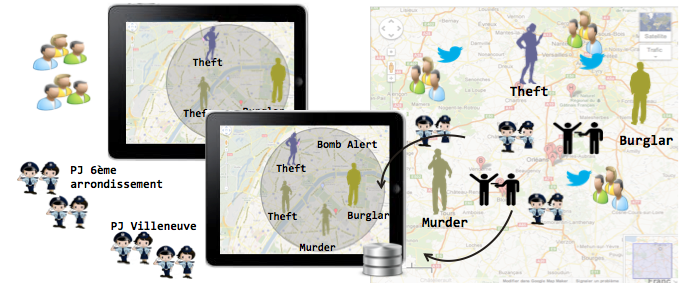
\includegraphics[width=0.95\textwidth]{figs/problem}}
%~ %add desired spacing between images, e. g. ~, \quad, \qquad etc. (or a blank line to force the subfig onto a new line)
%\\
%\subfloat[Contraints.]
{\label{fig:trans06}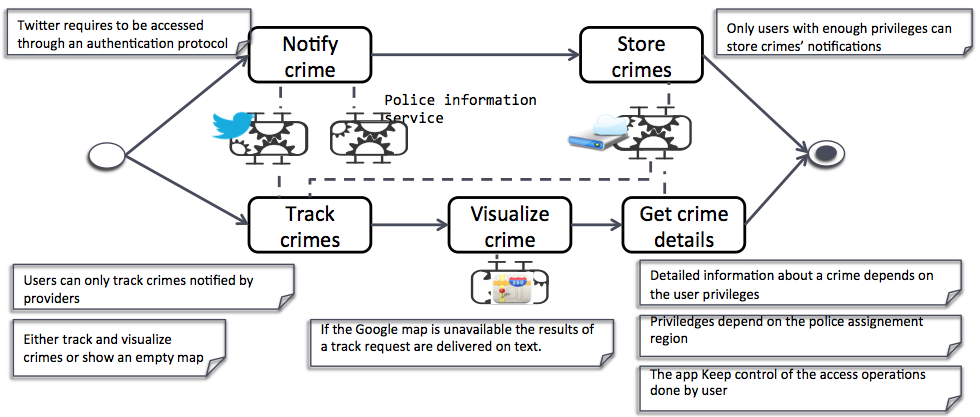
\includegraphics[width=0.95\textwidth]{figs/constraints}}
~ %add desired spacing between images, e. g. ~, \quad, \qquad etc. (or a blank line to force the subfig onto a new line)
\caption{Business process for the tracking crime example.}
\label{fig:constraints}
\end{figure}

In our example, crime processing can start with one of two tasks: \textit{(i) notify a crime}, or \textit{(ii) track a crime}.
Notified crimes are stored in a database. 
Tracked crimes are visualized in a map.
The used can ask for detailed information. 
The application is built upon four services: \textsf{twitter} and an \textsf{ad-hoc police service} for notifying crimes, \textsf{Amazon} used as  persistence service and  \textsf{Google Maps} for locating and displaying crimes on a map.

Non-functional requirements are specified by rules and conditions to be verified during the excecution of tasks.
In our example we have the following non-functional requirements:
\begin{trivlist}
\item[1.] Twitter requires to be accessed through an authentication protocol that allows three login failures before blocking. 
\item[2.] Crime notification needs privileged access.
\item[3.] Civilian users can only track crimes for which they have clearance: Civilian population cannot track all the crimes notified by the police. 
\item[4.] If \textsf{Google Maps} is unavailable, the results are delivered as text. 
\item[5.] Querying about crimes without having proper clearance yields an empty map.
\item[6.] Access rights to detailed information depends on user clearance and zone assignment for police officers. 
\item[7.] The application maintains a detailed log. 
\end{trivlist}

Considering the example of tracking crimes, all the system restrictions are
model as constraints in the methodology. We have three types of constraints:
\textit{value}, \textit{business} and \textit{exceptions behaviour} constraints.
Each use case can be associated to one or more constraints.

\paragraph*{\textit{$\pi$-UseCase} model:} 
In our example we have five use cases (Figure~\ref{fig:piUC}), which represent the
system functions (tasks) and constraints. 
We will not detail the functional part of the specification, due to lack of space.
The constrains defined for our tracking crime example are: 

\begin{trivlist}
  \item[-] The \textsf{Notify crime} task requires that the user is logged in. 
  This is an example of a \textit{value constraint}, where the value associated to the condition depends on the semantics of the application.
  In this case, it represents the maximmum number of allowed login attempts;
\item[-] The \textsf{Store crimes} task requires the verification of the user's clearance (also a value constraint). 
\item[-] In order to perform the \textsf{Track crimes} task, it is necessary that the notifier user is in the contact list of the requesting user.
This is an example of \textit{business constraint}.
Additionally the requesting user must be logged in.
\item[-]  For the \textsf{View Crime Map} task, the specification defines that if the Google Maps service is not available, the result is presented as text. This is an example of \textit{exceptional behaviour constraint}. 
The availability of the Google Maps service is verified by a \textit{business constraint}.
 \item[-] The \textsf{Show crime details} task is specified to have three constraints: A \textit{value constraint} is defined to verify the user's clearance level; A \textit{business constraint} is used to ensure that the user's clearance is valid for the geographic zone of the crime; Another \textit{value constraint} defines that the log is to be maintained.
\end{trivlist}
\begin{figure}[ht!]
\centering
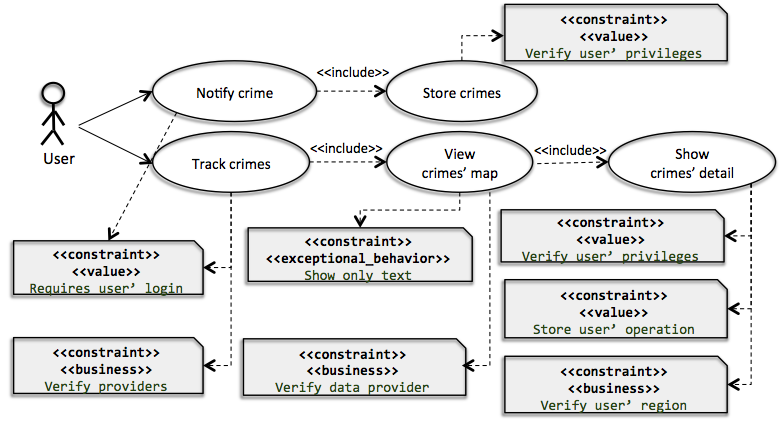
\includegraphics[width=0.8\textwidth]{figs/piUseCase}
\caption{$\pi$-UseCase Model}
\label{fig:piUC}
\end{figure}
\paragraph*{\textit{$\pi$-ServiceProcess} model:}
The model presented in Figure~\ref{fig:piUC} is transformed, at this stage of the development, into a similar graph, where \textit{(i)} the task nodes are better detailed, by refining the control and data flows; and \textit{(ii)} constraints are transformed into \textit{contracts} (pre- and post-conditions).
The new model describes the application's activities and defines contracts for each activity or for parts of the application.

A model-to model transformation is defined in order refine the \textit{$\pi$-UseCase} model of the application into the more detailed model. 
This (semi-automatic) transformation process is supported by a tool (described in~\cite{SouzaNeto:2012}).

The \textit{$\pi$-ServiceProcess} model defined for our tracking crime application is presented in Figure~\ref{fig:piSP}, where: 
\begin{enumerate}
\item Tasks of the previous model are transformed into \textit{actions};
\item Actions are grouped into \textit{activities} (in accordance to the business logic).
\item Constraints of the \textit{$\pi$-UseCase} model are transformed into assertions.
\end{enumerate}

\begin{figure}[ht!]
\centering
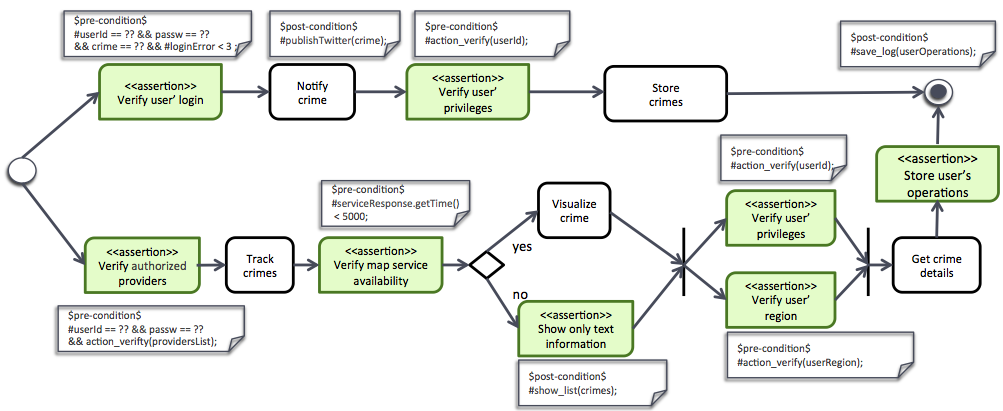
\includegraphics[width=0.99\textwidth]{figs/piServiceProcess}
\caption{$\pi$-\textit{ServiceProcess} Model}
\label{fig:piSP}
\end{figure}

\paragraph*{\textit{$\pi$-ServiceComposition} model:} 
This model refines the previous model by using the activities to produce the workflow of the application.
The model serves to identify those entities that collaborate with the service process by providing services to execute actions. 
This model identifies the services and functions that correspond to each action in the business process.

\begin{figure}[t]
\centering
\subfloat[$\pi$-ServiceComposition Model]
{\label{fig:piSC}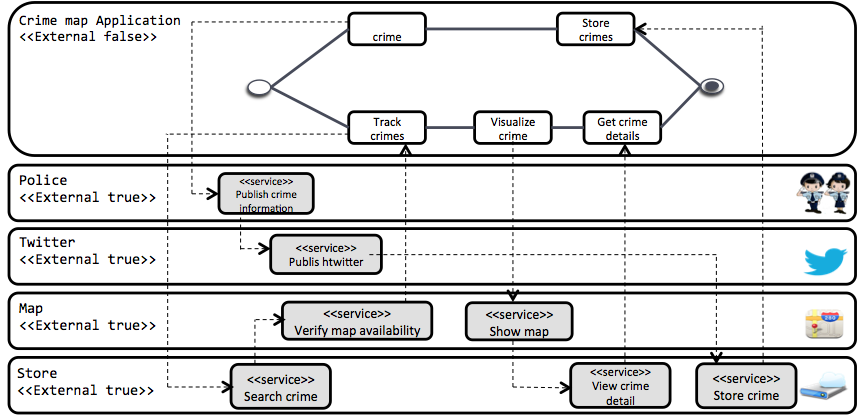
\includegraphics[width=0.95\textwidth]{figs/piServiceComposition}}
~ %add desired spacing between images, e. g. ~, \quad, \qquad etc. (or a blank line to force the subfig onto a new line)
\\
\subfloat[$\pi$-ServiceComposition Policies]
{\label{fig:crimePolicies}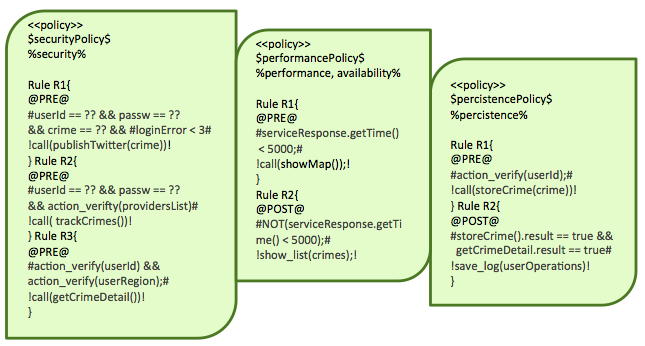
\includegraphics[width=0.85\textwidth]{figs/policies}}
~ %add desired spacing between images, e. g. ~, \quad, \qquad etc. (or a blank line to force the subfig onto a new line)
\caption{Service Composition and Policies.}
\label{fig:policies}
\end{figure}
This model describes the service compositions and their related business
collaborators (external services), policies, rules associated with a policy and
the whole application process and functionalities.
The workflow execution will consider the composition of business services and
their specific Business Collaborators. 
Each action will trigger the execution of one or more external services. 
Before and after each service call, policy rules are verified.

In the case of our crime tracking example, the model produced from the $\pi$-\textit{ServiceProcess} model of Figure~\ref{fig:piSP} is given in Figures~\ref{fig:piSC} and~\ref{fig:crimePolicies}.
Figure~\ref{fig:piSC} shows how the crime application interacts with its \textit{busines collaborators} (external services and entities).
The interaction occurs by means of function calls (denoted by dotted lines in the figure).
Figure~\ref{fig:crimePolicies} shows the definition of three \textit{policies}, which define rules for service execution.
In our case we have policies for \textit{Security}, \textit{Performance} and \textit{Persistence}. 


\paragraph*{$\pi$\textit{-PEWS} Model:}
These models are produced by a model-to-text transformation that takes a $\pi$-\textit{ServiceComposition} model and generates $\pi$-\textit{PEWS} specification code.
This code is a service composition program that can be compiled into executable code.
$\pi$-\textit{PEWS} models are expressed in a variant of the PEWS composition language.

\begin{figure}[t]
\footnotesize
%\begin{lstlisting}[label=list:rulePre,caption=ATL - piServiceComposition2piPEWS : Pre-condition Rule. ]
%\begin{lstlisting}[label=list:rulePre]
\begin{verbatim}
//Namespaces specify service URI
1 namespace twitter = www.twitter.com/service.wsdl
2 namespace googlemaps = maps.googleapis.com/maps/api/service
3 namespace amazondynamodb = rds.amazonaws.com/doc/2010-07-28/AmazonRDSv4.wsdl
4 namespace police = www.police.fr/service.wsdl

//Operations 
5 alias publishTwitter = portType/publishTwitter in twitter
6 alias searchCrime = portType/searchCrime in amazondynamodb 
7 alias showMap = portType/showMap in googlemaps 
...
//Services
8  service notifyCrime = publishCrime  . publishTwitter 
9  service trackCrime= searchCrime . verifyService
10 Service visualizeCrime =  showMap . getCrimeDetail
...
//Path
11 ( notifyCrime . storeiCrime ) || 
12 ( trackCrime . visualizeCrime . getCrimeDetail )
...
//Contracts
13 defContract notifyCrimeContract{
14	isAppliedTo: notifyCrime
15	requires: userId == ?? && passw == ?? && 
16	                               req(notifyCrime)  < 3
17 	  (OnFailureDo: NOT(action_publish(crime));
18	ensures: publishTwitter(crime) == true
19 	  (OnFailureDo: skip);
20 }
...
\end{verbatim}
% \end{lstlisting}
\caption{$\pi$-PEWS code for the crime tracking example (partial, simplified).\label{fig:pewscontract} }
\end{figure}

The $\pi$-PEWS program generated from the model in Figure~\ref{fig:policies} is partially presented in Figure~\ref{fig:pewscontract}. 
The figure shows a simplified program code, produced in accordance to the following guidelines:
\begin{trivlist}
\item[1.] Namespaces, identifying the addresses of external services are produced from the Business Collaborators of the higher-level model. 
We define four of them, corresponding to the Police, Twitter, Google Map and Amazon partners.
\item[2.] Specific operations exported by each business collaborator are identified to an \textit{operation} of the program (Each operation is given an \texttt{alias}).
\item[3.] The workflow in Figure~\ref{fig:piSC} is translated into a textual representation (lines 11 and 12 of the program).
\item[4.] \textit{Contracts} are defined in $\pi$-PEWS as having pre-conditions (\texttt{requires}), post-conditions (\texttt{ensures}) and actions (\texttt{OnFailureDo}) to be executed in the case thar a condition is not verified. 
Contracts are generated from Policies (such as those of Figure~\ref{fig:piSC}.
\end{trivlist}


For a more comprehensive account of $\pi$SOD-M the reader can refer to~\cite{SouzaNeto:2012}.


\section{Related Work and Conclusions}
\label{sec:conclusions}

Over the last years, a number of approaches have been proposed for the
development of web services. These approaches range from the proposal of new 
languages for web service descriptions~\cite{bpel03,SBS04} 
to techniques to support phases of the development cycle of this kind of
software~\cite{lipari2007,BianculliGSBG07}. In general, these
approaches concentrate on specific problems, like supporting transactions or
QoS, in order to improve the security and reliability of service-based
applications. Some proposals address service composition: workflow
definition~\cite{AalstHKB03,MuP06} or semantic equivalence between
services~\cite{BHM06}. The proposed solutions come from many communities, 
including those of Theoretical Computer Science~\cite{VA05,GGP08}, 
Software Engineering~\cite{Aal03,MendesPDB09}, Programming
Languages~\cite{MPC08,bpel03} and Databases~\cite{ABM01}.

Despite the variety of tecniques proposed, there is not yet a consensus on a software
process methodology for web services. Some methodologies address the service-based 
development towards a standard or a new way to develop reliable applications. 
SOD-M and SOMF \cite{somf} are MDD approaches for web services; 
S-Cube \cite{scube2010book} is focused on the representation of business processes and 
service-based development; SOMA \cite{soma} is a methodology described by IBM
for SOA solutions; Extended SOA \cite{PapazoglouH06} merges RUP and
BPM\cite{bpm} concepts for service modeling; DEVISE \cite{DEVISE} is a
methodology for building service-based infrastructure for collaborative
enterprises. Other proposals include, the WIED model \cite{TongrungrojanaL04}, 
that acts as a bridge between business modeling and design models, and traditional 
approaches for software engineering \cite{sommerville08} applied to SOC. 

\bigskip

This paper presented the $\pi$SOD-M software process for specifying and designing service based applications in the presence of some non-functional constraints. 
Our proposal harness the SOD-M method with constraints, policies and contracts in order to consider non-functional constraints.
We implemented the proposed meta-models on the Eclipse platform and we illustrated the approach by developping a simple application.

$\pi$SOD-M is being used in an academic environment.
So far, the preliminary results indicate that $\pi$SOD-M approach is useful for the development of complex web service applications. 
We are now working on the definition of a PCM-level meta-model to generate BPEL programs (instead of $\pi$-PEWS). 
   
\bibliographystyle{splncs_srt}
\bibliography{biblio2} 
\end{document}
